\documentclass[border=10pt]{standalone}
\usepackage{tikz}
\usepackage{amsmath}
\usetikzlibrary{arrows.meta}

% ========== 书内统一配色 ==========
\definecolor{inFill}{RGB}{183,224,177}
\definecolor{inLine}{RGB}{32,102,32}
\definecolor{hidFill}{RGB}{199,203,243}
\definecolor{hidLine}{RGB}{52,58,143}
\definecolor{outFill}{RGB}{243,199,199}
\definecolor{outLine}{RGB}{143,52,52}
\definecolor{biasFill}{RGB}{255,241,194}
\definecolor{biasLine}{RGB}{171,122,34}
\definecolor{opFill}{RGB}{250,250,250}
\definecolor{opLine}{RGB}{70,70,70}
\definecolor{lineC}{RGB}{38,44,110}
\colorlet{head}{red!60!black}

\begin{document}
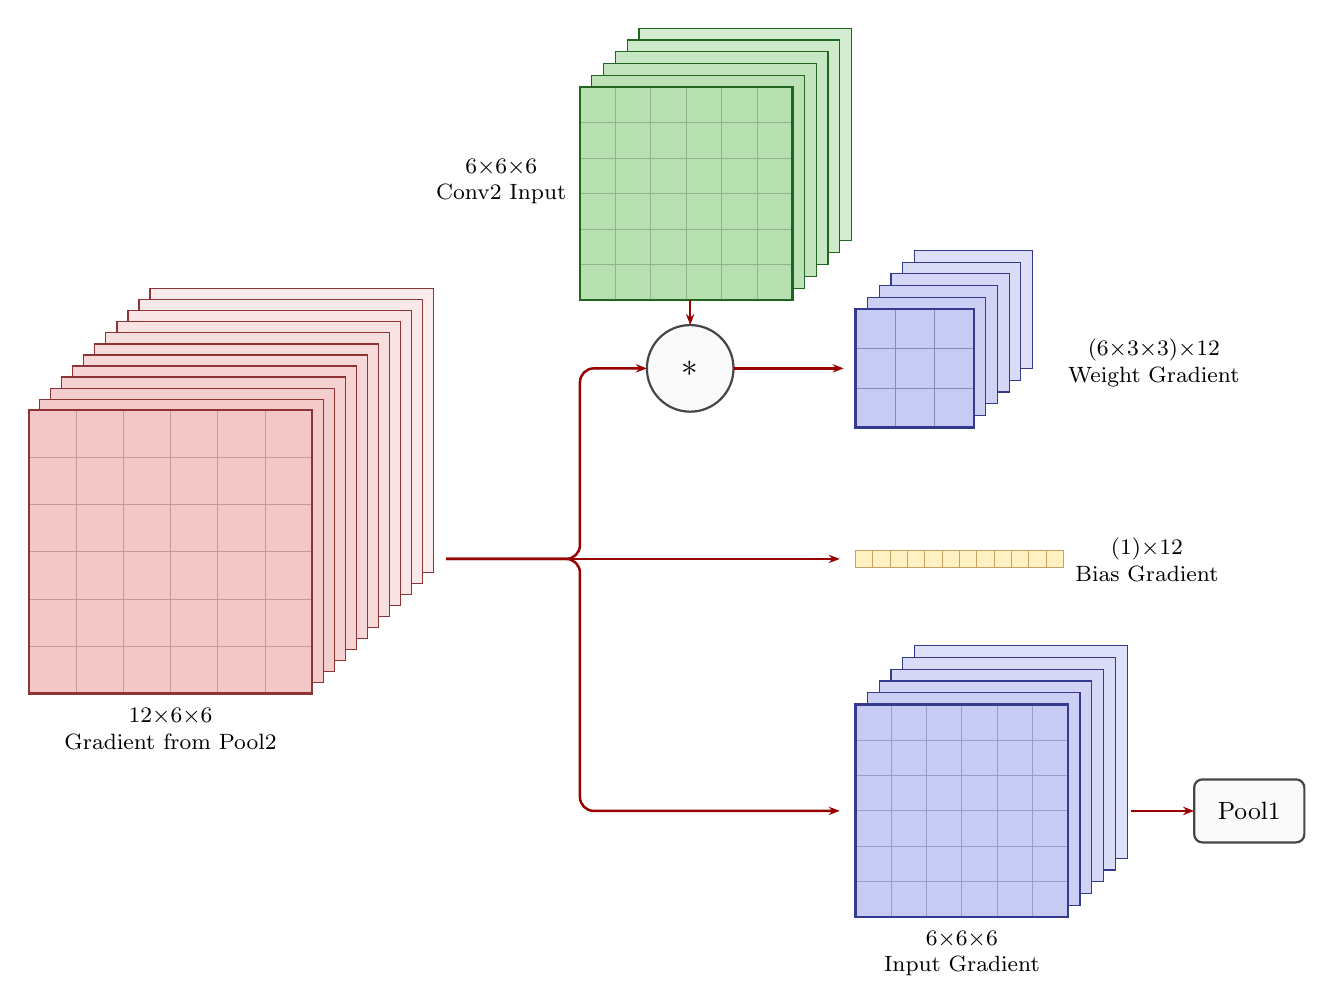
\begin{tikzpicture}[>={Stealth[length=4pt]}, line width=0.8pt, font=\small,
    every node/.style={inner sep=0pt, outer sep=0pt, align=center},
    rbox/.style={draw=opLine, fill=opFill, rounded corners=3pt,
                 minimum width=1.4cm, minimum height=0.8cm, font=\small}]

  % ================= 左：上游梯度（红，12 层） =================
  \foreach \k in {11,10,...,1}{
    \pgfmathtruncatemacro{\op}{100-6*\k}
    \fill[outFill!\op, draw=outLine, line width=0.4pt]
          ({0.14*\k},{1.0+0.14*\k}) rectangle ++(3.6,3.6);
  }
  \fill[outFill] (0,1.0) rectangle (3.6,4.6);
  \draw[outLine!50, line width=0.3pt, shift={(0,1.0)}, step=0.6] (0,0) grid (3.6,3.6);
  \draw[outLine] (0,1.0) rectangle (3.6,4.6);
  \node[font=\footnotesize] at (1.8,0.55) {12$\times$6$\times$6\\Gradient from Pool2};

  % ================= 上：前向输入 X（绿） =================
  \foreach \k in {5,4,...,1}{
    \pgfmathtruncatemacro{\op}{100-8*\k}
    \fill[inFill!\op, draw=inLine, line width=0.4pt]
          ({7.0+0.15*\k},{6.0+0.15*\k}) rectangle ++(2.7,2.7);
  }
  \fill[inFill] (7.0,6.0) rectangle (9.7,8.7);
  \draw[inLine!50, line width=0.3pt, shift={(7.0,6.0)}, step=0.45] (0,0) grid (2.7,2.7);
  \draw[inLine] (7.0,6.0) rectangle (9.7,8.7);
  \node[font=\footnotesize] at (6.0,7.5) {6$\times$6$\times$6\\Conv2 Input};

  % ================= 星号操作符（★ 只要圆形） =================
  \node[circle, draw=opLine, fill=opFill, minimum size=1.1cm,
        inner sep=0pt, font=\large] (corr) at (8.4,5.13) {$\ast$};

  % ---- input → 星号（垂直向下，从北面进入） ----
  \draw[head, ->, line width=0.9pt] (8.4,6.0) -- (8.4,5.68);

  % ================= 三条独立完整箭头（无文字标签） =================
  % ---- 箭头 1：上游 → 星号（右→上→右，从西面进入） ----
  \draw[head, ->, line width=0.9pt, rounded corners=5pt]
        (5.3,2.71) -- (7.0,2.71) -- (7.0,5.13) -- (7.85,5.13);
  % ---- 箭头 2：上游 → 偏置梯度（直右） ----
  \draw[head, ->, line width=0.9pt] (5.3,2.71) -- (10.3,2.71);
  % ---- 箭头 3：上游 → 输入梯度（右→下→右） ----
  \draw[head, ->, line width=0.9pt, rounded corners=5pt]
        (5.3,2.71) -- (7.0,2.71) -- (7.0,-0.49) -- (10.3,-0.49);

  % ---- 星号 → 权重梯度（水平向右） ----
  \draw[head, ->, line width=0.9pt] (8.95,5.13) -- (10.35,5.13);

  % ================= 右竖排 1：权重梯度（x=10.5） =================
  \foreach \k in {5,4,...,1}{
    \pgfmathtruncatemacro{\op}{100-8*\k}
    \fill[hidFill!\op, draw=hidLine, line width=0.4pt]
          ({10.5+0.15*\k},{4.38+0.15*\k}) rectangle ++(1.5,1.5);
  }
  \fill[hidFill] (10.5,4.38) rectangle (12,5.88);
  \draw[hidLine!60, line width=0.3pt, shift={(10.5,4.38)}, step=0.5] (0,0) grid (1.5,1.5);
  \draw[hidLine] (10.5,4.38) rectangle (12,5.88);
  \node[font=\footnotesize, anchor=west] at (13.2,5.2)
        {(6$\times$3$\times$3)$\times12$\\Weight Gradient};

  % ================= 右竖排 2：偏置梯度（x=10.5） =================
  \foreach \i in {0,...,11}
    \draw[biasLine!70, fill=biasFill, line width=0.4pt]
          ({10.5+0.22*\i},2.6) rectangle ++(0.22,0.22);
  \node[font=\footnotesize] at (14.2,2.7) {(1)$\times$12\\Bias Gradient};

  % ================= 右竖排 3：输入梯度（x=10.5） =================
  \foreach \k in {5,4,...,1}{
    \pgfmathtruncatemacro{\op}{100-8*\k}
    \fill[hidFill!\op, draw=hidLine, line width=0.4pt]
          ({10.5+0.15*\k},{-1.84+0.15*\k}) rectangle ++(2.7,2.7);
  }
  \fill[hidFill] (10.5,-1.84) rectangle (13.2,0.86);
  \draw[hidLine!50, line width=0.3pt, shift={(10.5,-1.84)}, step=0.45] (0,0) grid (2.7,2.7);
  \draw[hidLine] (10.5,-1.84) rectangle (13.2,0.86);
  \node[font=\footnotesize] at (11.85,-2.3) {6$\times$6$\times$6\\Input Gradient};

  % ================= 输入梯度 → Pool1 =================
  \node[rbox] (p1) at (15.5,-0.49) {Pool1};
  \draw[head, ->, line width=1pt] (14.0,-0.49) -- (p1.west);

\end{tikzpicture}
\end{document}